\twocolumn[
\begin{center}
\title{\color[cmyk]{1, 0.57, 0, 0.38}{\Huge\bfseries Fedora 17\\}} % definisco il titolo dell'articolo
\author{\scriptsize Robert Mayr (robyduck@fedoraonline.it)} % definisco l'autore e altre informazioni
\date{}
\end{center}
{\color[cmyk]{1, 0.46, 0, 0}\LARGE Fedora 17 - una panoramica sulle novità}\\
\maketitle
\normalsize
\doublespacing
\hfill
]
\onehalfspacing
\lettrine[lines=1, loversize=0.1, lraise=0.1]{\color[cmyk]{0.5, 0, 1, 0}\bfseries E'}{} notizia di pochi giorni fa l'annuncio di {\itshape Dennis Gilmore} riguardante l'uscita della versione {\itshape alpha} di Fedora 17 ``Beefy Miracle'', per la quale sono previste le caratteristiche che possiamo vedere complete a questo indirizzo: {\itshape http://fedo\\raproject.org/wiki/Releases/17/Feature\\List\#Fedora\_17\_Accepted\_Features}.\\

La roadmap per il rilascio della versione {\itshape stable} si può trovare alla pagina {\itshape http://\\fedoraproject.org/wiki/Schedule}.\\

\begin{figure}[htbp]
\centering
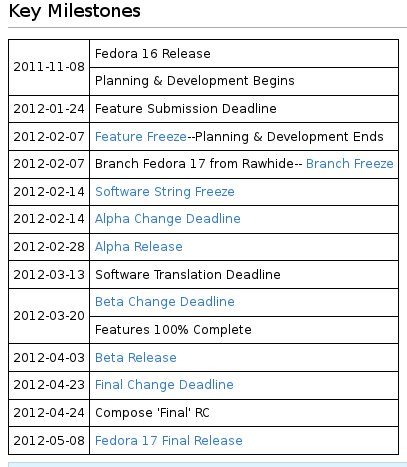
\includegraphics[scale=.60]{articoli/notizie/immagini/roadmap_wiki.jpeg}
\caption{roadmap per Fedora 17 {\itshape Beefy Miracle}}
\end{figure}


Come al solito la lista delle features accettate è molto differenziata, ma tra queste possiamo rilevarne alcune molto importanti sia per gli utenti finali che per chi è interessato al sistema ed allo sviluppo:
\begin{itemize}
\item Gnome 3.4.
\item KDE 4.8.
\item Gimp 2.8.
\item Kernel 3.3.
\item GCC 4.7.x.
\item PHP 5.4.
\item Software rendering for gnome-shell.
\item Move all to /usr.
\item ABRT Backtrace Deduplication Service.
\item Eucalyptus.
\item Firewalld.
\item KVM Live Block Migration.
\item NetworkManager Hotspots.
\item Riak.
\end{itemize}

Vediamone alcune più dettagliatamente:\\

\begin{center}
{\centering\bfseries Gnome 3.4}
\end{center}
Tra le novità spicca, anche se ancora in fase di sviluppo e con qualche ostacolo di trademark, {\itshape Boxes} che sempificherà l'accesso ad altri sistemi operativi, siano essi fisici, virtuali o raggiungibili via rete. Sarà incluso anche l'accesso remoto, il tutto utilizzando la tecnologia Qemu. Nonostante lo sviluppo di virt-manager {\itshape Boxes} si pone l'obiettivo di mettere a disposizione dell'utente un'interfaccia più amichevole.

\begin{figure}[!h]
\centering
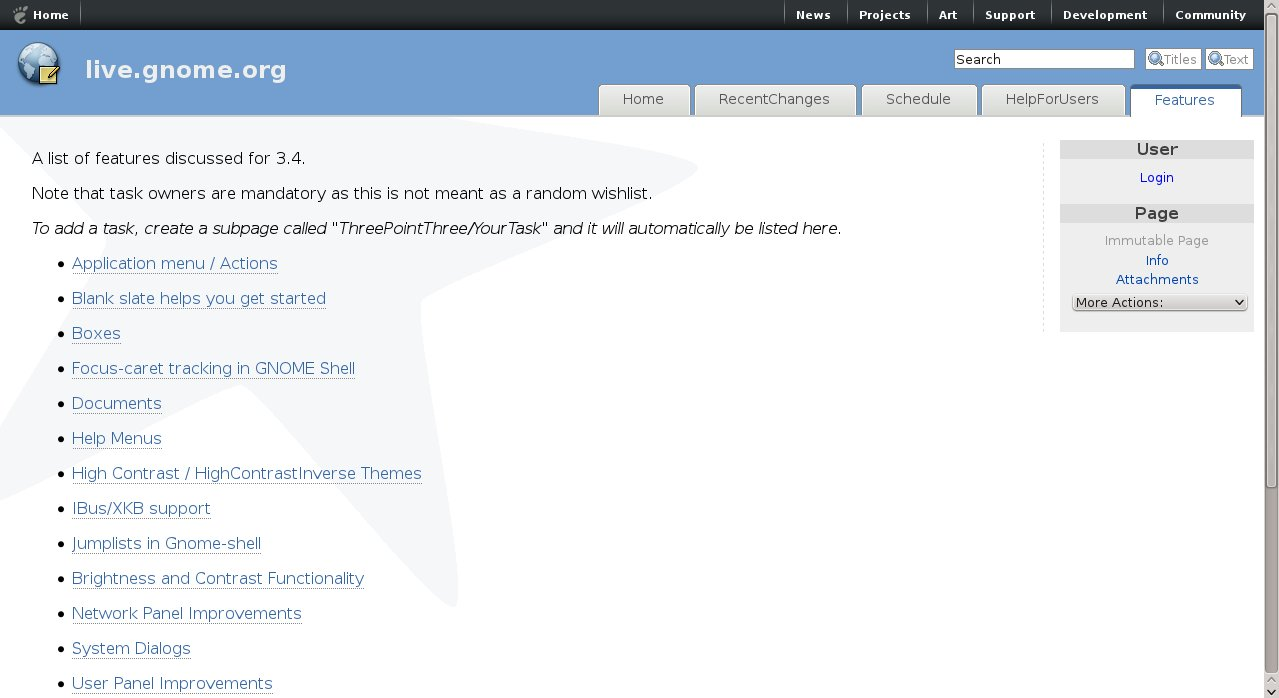
\includegraphics[scale=.20]{articoli/notizie/immagini/gnome_3_4.jpeg}
\caption{live.gnome.org}
\end{figure}
\begin{center}
{\centering\bfseries KDE 4.8}
\end{center}
In questa versione, l'utility{\itshape KDE Power Management System Settings} è stata aggiornata sia per quanto riguarda l'interfaccia utente che per il layout. Sono stati introdotti miglioramenti per {\itshape Dolphin}, {\itshape Gwenview}, {\itshape KMail} (non si dovrebbero riscontrare i problemi di sicurezza e stabilità delle versioni precedenti), {\itshape Kate} e molto altro.

\begin{figure}[htbp]
\centering
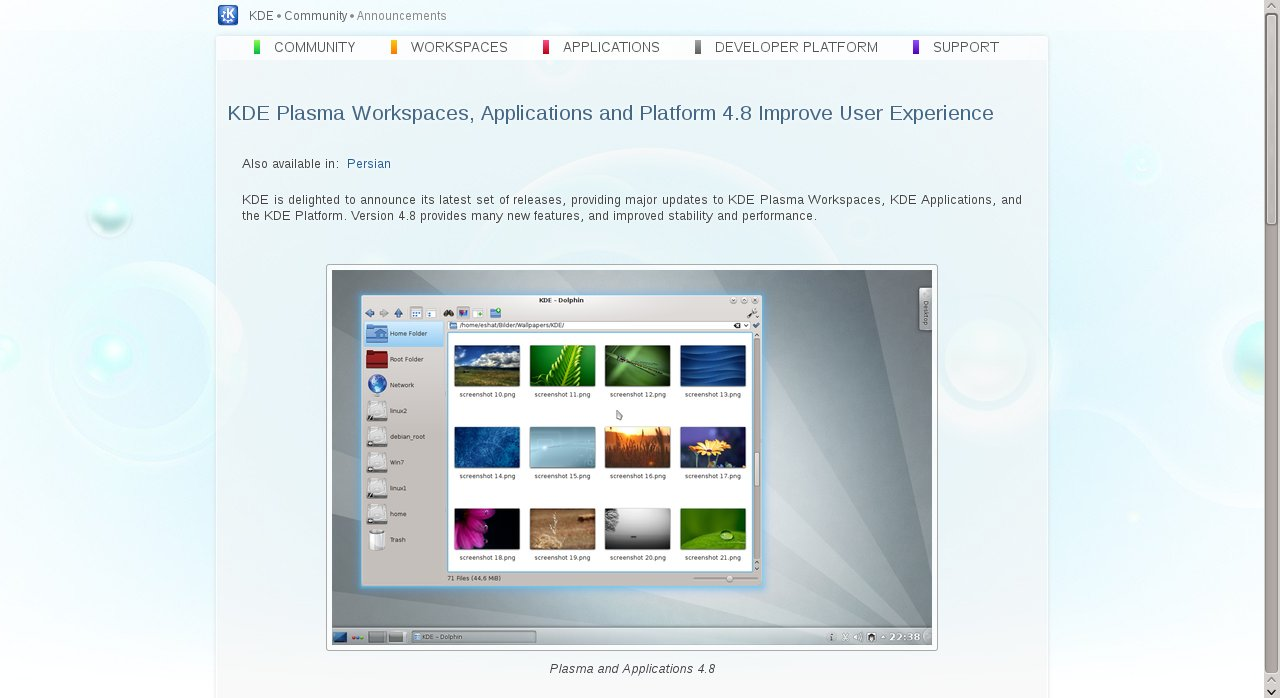
\includegraphics[scale=.20]{articoli/notizie/immagini/kde_4_8.jpeg}
\caption{kde.org}
\end{figure}

\begin{center}
{\centering\bfseries Kernel 3.3}
\end{center}
Uno dei cambiamenti nella versione 3.3 del kernel è dovuto all'inserimento di un nuovo meccanismo per regolare la dimensione dei filesystems ext4; questo meccanismo dovrebbe ora lavorare più velocemente. Miglioramenti sono stati apportati anche per l'audio HDMI su tipologie di chipset AMD e Nvidia. Sono stati raggruppati, inoltre, alcuni dispositivi ethernet in un unico dispositivo virtuale. E' stato inserito il supporto a Open vSwitch. Il filesystem btrfs è stato ottimizzato per operazioni con volumi RAID ed è inserita in via sperimentale la verifica dell'integrità dei dischi in alcune operazioni.

\begin{figure}[htbp]
\centering
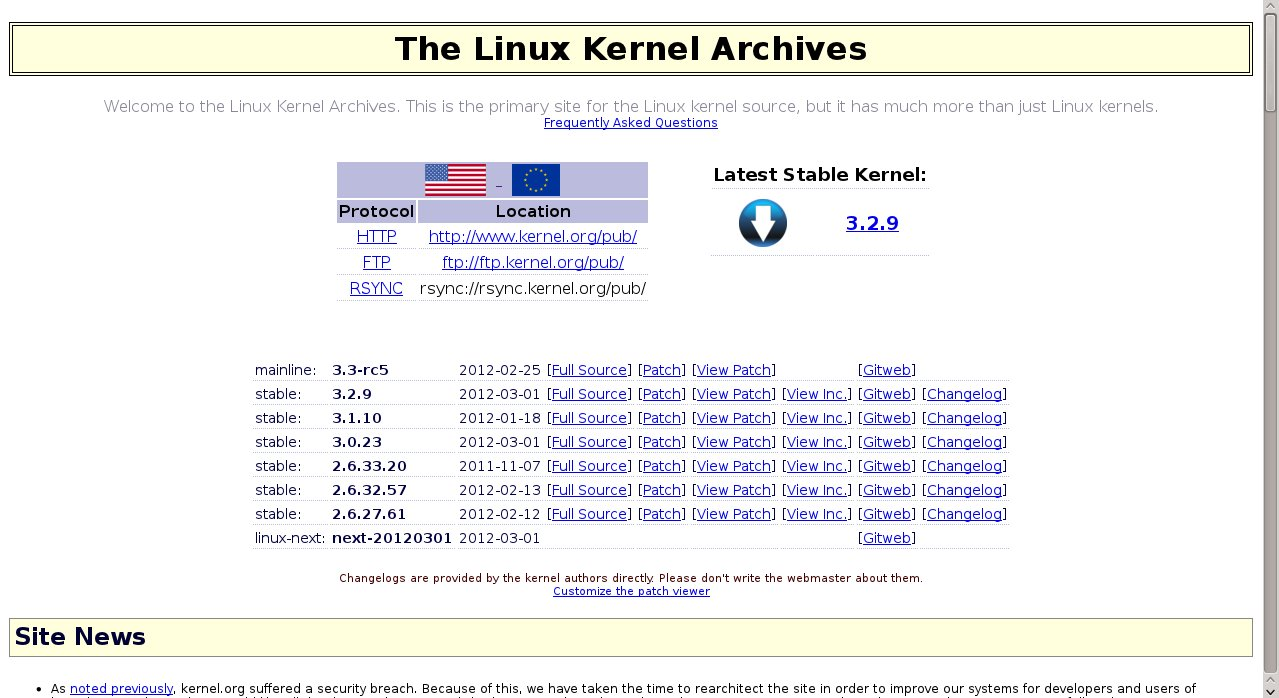
\includegraphics[scale=.20]{articoli/notizie/immagini/kernel.jpeg}
\caption{kernel.org}
\end{figure}

\begin{center}
{\centering\bfseries Software rendering for gnome-shell}
\end{center}
Gnome-shell sarà in grado di funzionare anche con gran parte di quelle schede grafiche che non supportano l'accelerazione 3D, un enorme passo avanti per quanto riguarda l'usabilità del DE di default.

\begin{center}
{\centering\bfseries Move all to /usr}
\end{center}
Come già visto nell'articolo relativo ai pacchetti rpm, è stato stabilito lo spostamento di tutte le /lib e /bin sotto la directory /usr. Di fatto, le directory /lib, /lib64, /bin e /sbin conterranno soltanto dei link simbolici ai file che si troveranno sotto la directory /usr.

\begin{center}
{\centering\bfseries ABRT Backtrace Deduplication Service}
\end{center}
Durante l'inserimento di un nuovo bug nel RedHat Bugzilla, ABRT controllerà se ne è già stato aperto uno per lo stesso problema, onde evitare duplicati.

\begin{center}
{\centering\bfseries Eucalyptus}
\end{center}
Eucalyptus è un software cloud computing per l'utilizzo privato, che permette di utilizzare le infrastrutture esistenti per creare clouds per computer, memoria di massa e rete. Nelle novità del cloud computing si inserisce anche il toolkit OpenNebula.

\begin{center}
{\centering\bfseries Firewalld - default firewall solution}
\end{center}
Il nuovo firewall di default sostituisce i servizi iptables, iptables-ipv6 e ebtables.

\begin{center}
{\centering\bfseries KVM Live Block Migration}
\end{center}
KVM avrà la possibilità di migrare immagini del disco, mentre questo è in "funzione" (live block migration). oVirt è ancora in fase sperimentale, ma dovrebbe essere in grado di virtualizzare server, fare migrazioni live block e molto altro.

\begin{center}
{\centering\bfseries NetworkManager Hotspots}
\end{center}
Questa aggiunta mette NetworkManager nelle condizioni di funzionare come Access Point.

\begin{center}
{\centering\bfseries Riak}
\end{center}
Il database in clustering NoSQL viene incluso nei repo di Fedora. Riak avrà anche una consolle di amministrazione dei cluster, che rende più agevole la loro gestione.\\

Per concludere, un'ultima notizia: il filesystem di default rimarrà ext4 (il quale avrà il supporto per gestire dischi oltre i 16TB) in quanto btrfs è slittato, per alcune incompatibilità e restrizioni di anaconda, almeno alla versione 18.\\

Il resto lo scopriremo all'uscita di {\bfseries Fedora 17 ``Beefy Miracle''} l' 8 Maggio 2012, salvo ritardi.\\
